\subsection{Progettazione architetturale}
Questa fase comincia subito dopo la presentazione e finisce con la data di consegna per la Revisione di Progettazione, ovvero dal 18/01/2020 al 01/03/2021.\\
In questo periodo verrà individuata una soluzione architetturale che funga da sostegno per l'implementazione del prodotto. Deve soddisfare tutti i requisiti richiesti, oltre ad essere facilmente comprensibile ed attuabile. 
\begin{itemize}
\item \textbf{Incremento e verifica dei documenti:} se fosse necessario, i documenti prodotti dal team verranno integrati.

 \item \glo{\textbf{Technology baseline}}: Viene fatta un'analisi ad alto livello per comprendere le tecnologie coinvolte, in due passi distinti:
\begin{itemize}
 \item \textbf{decomposizione del prodotto} in parti, in modo da essere realizzato con risorse sostenibili e costi compatibili;
 \item \textbf{analisi delle componenti individuate}, in modo da determinare come ciascuna interagisce con le altre.  
\end{itemize}
L'architettura verrà progettata sulla base di \glo{design patterns} esistenti e verrà realizzato un \glo{\textit{Proof of Concept}} da condividere con il proponente, che dimostra adeguatezza e fattibilità in modo coerente agli obiettivi. In particolare, poiché il \textit{PoC} rappresenta una baseline per lo sviluppo, riguarderà due incrementi:
\begin{itemize}
	\item \textbf{Incremento 0}: questo periodo, che va dal 08/02/2020 al 17/02/2020, si focalizza su una prima bozza dell'\glo{UI} e ha l'obbiettivo d'implementare il caricamento dei dati nel sistema attraverso un file del tipo csv e la selezione delle dimensioni da utilizzare. \textbf{[aggiungere riferimenti agli UC]}
	\item \textbf{Incremento 1}: questo periodo, che va dal 16/02/2020 al 24/02/2020, è dedicato allo studio approfondito della libreria \glo{D3.js} è sull'implementazione della visualizzazione \glo{Scatter Plot Matrix} senza però la possibilità di personalizzazione. \textbf{[aggiungere riferimenti agli UC]}
\end{itemize} 

\end{itemize}

\subsubsection{Periodi}
La pianificazione di questa fase è stata organizzata nel modo seguente:
\begin{itemize}
\item \textbf{25/01/2020 - 08/02/2020}: a causa della concomitanza con la sessione accademica, il team ha fissato la prima \glo{milestone} al termine di questo periodo. Alla scadenza, il gruppo dovrà aver iniziato lo studio delle tecnologie per la Technology baseline, oltre ad aver controllato buona parte della documentazione.

\item \textbf{08/02/2020 - 18/02/2020}: il secondo periodo ha una milestone fissata per il giorno 18, il team s'impegnerà a terminare i lavori avviati nel periodo precedente. Inoltre l'obbiettivo è terminare il primo incremento previsto per il \textit{Proof of Concept}.

\item \textbf{18/02/2020 - 01/03/2020}: in questo periodo che termina con la consegna dell'1, il gruppo prevede di terminare anche il secondo incremento relativo al \textit{Proof of Concept} e ultimato le verifiche.
\end{itemize}

\subsubsection{Diagramma di Gantt: Progettazione architetturale}
\begin{figure}[h]
	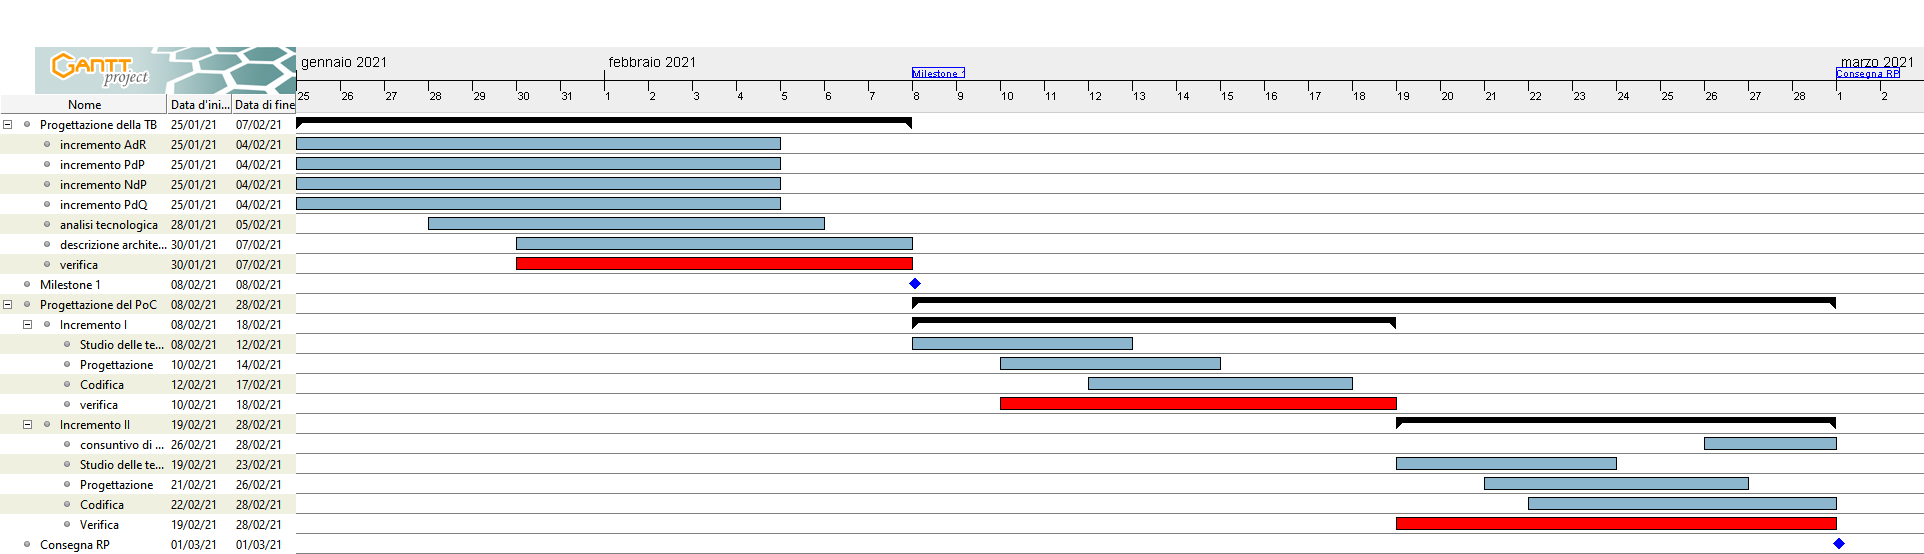
\includegraphics[scale=0.30]{Images/GanttPianificazioneProgettazioneArchitetturale.PNG}
	\caption{Diagramma di Gantt dell'attività di Progettazione Architetturale}
\end{figure}